% Figure: the full pipeline with responsibility groups (part 10).
% Build: pdflatex pipeline.tex  (run inside figures/)
\documentclass[tikz,border=6pt]{standalone}
\usetikzlibrary{positioning,arrows.meta,fit,backgrounds}
\begin{document}
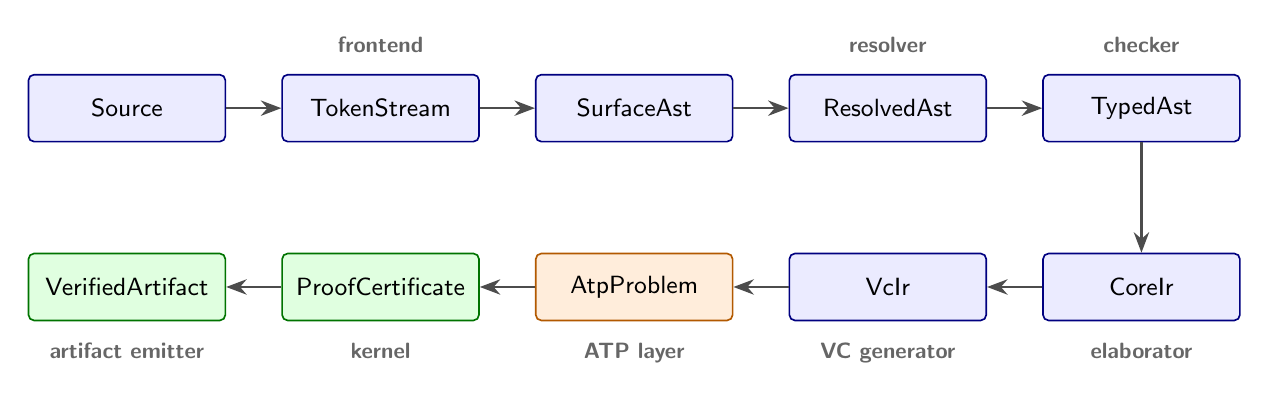
\begin{tikzpicture}[
  font=\sffamily,
  art/.style={draw, rounded corners=2pt, align=center, minimum height=8.5mm,
              minimum width=25mm, line width=0.6pt, fill=blue!8, draw=blue!50!black,
              font=\sffamily\small},
  group/.style={font=\sffamily\footnotesize\bfseries, text=black!60},
  flow/.style={-{Stealth[length=2.6mm]}, line width=0.9pt, black!70},
  node distance=4mm and 7mm,
]
  % Row 1
  \node[art] (src) {Source};
  \node[art, right=of src] (tok) {TokenStream};
  \node[art, right=of tok] (sur) {SurfaceAst};
  \node[art, right=of sur] (res) {ResolvedAst};
  \node[art, right=of res] (typ) {TypedAst};
  % Row 2
  \node[art, below=14mm of typ] (core) {CoreIr};
  \node[art, left=of core] (vc) {VcIr};
  \node[art, left=of vc, fill=orange!14, draw=orange!70!black] (prob) {AtpProblem};
  \node[art, left=of prob, fill=green!12, draw=green!45!black] (cert) {ProofCertificate};
  \node[art, left=of cert, fill=green!12, draw=green!45!black] (ver) {VerifiedArtifact};

  \draw[flow] (src) -- (tok);
  \draw[flow] (tok) -- (sur);
  \draw[flow] (sur) -- (res);
  \draw[flow] (res) -- (typ);
  \draw[flow] (typ) -- (core);
  \draw[flow] (core) -- (vc);
  \draw[flow] (vc) -- (prob);
  \draw[flow] (prob) -- (cert);
  \draw[flow] (cert) -- (ver);

  % Responsibility groups
  \node[group, above=1.5mm of tok] {frontend};
  \node[group, above=1.5mm of res] {resolver};
  \node[group, above=1.5mm of typ] {checker};
  \node[group, below=1.5mm of core] {elaborator};
  \node[group, below=1.5mm of vc] {VC generator};
  \node[group, below=1.5mm of prob] {ATP layer};
  \node[group, below=1.5mm of cert] {kernel};
  \node[group, below=1.5mm of ver] {artifact emitter};
\end{tikzpicture}
\end{document}
